{\color{oorange}\subsection{Metodo del Gradiente e Metodo del Gradiente Coniugato a confronto}}

\begin{algorithm}[H]
	\caption*{Metodo di discesa generale in \code{pseudocode}}\label{alg:mg}
	\begin{algorithmic}[1]
		\State $x_0 \in R^n, k=0$
        \While{$\nabla f(x_k) \neq 0$ and $k <$ maxit}\Comment{maxit è il massimo numero di iterazioni}
            \State calcolare la direzione di discesa $d_k$ (infulenzato da $\nabla f(x_k)$)
            \State calcolare il passo di discesa $\alpha_k$
            \State $x_{k+1} = x_k+\alpha_kd_k$
            \State $k = k+1$
        \EndWhile
        \State \Return $x_{last}$
	\end{algorithmic}
\end{algorithm}

Analizziamo il comportamento del gradiente utilizzando i due metodi sull'immagine data.camera():
\begin{figure}[H]
    \centering
    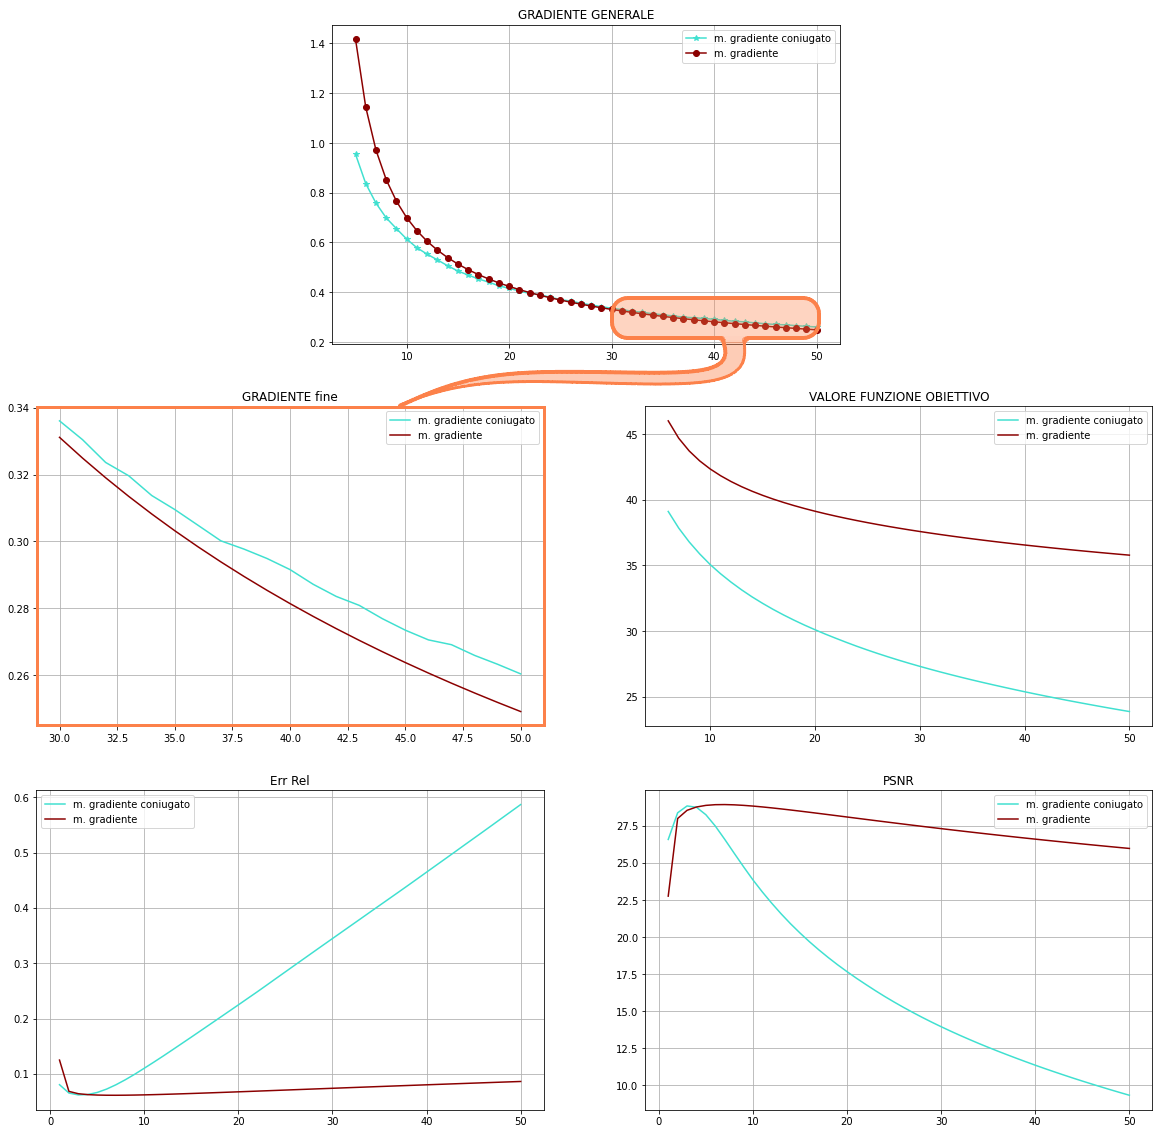
\includegraphics[width=\textwidth]{output/MGCvsMG-enph.png}
    \caption{Gradiente immagine data.camera()}
    \label{fig:MGCvsMGdatacamera}
\end{figure}

Per quanto riguarda l'immagine fotografica pugile.png, abbiamo riscontrato: 

\begin{figure}[H]
    \centering
    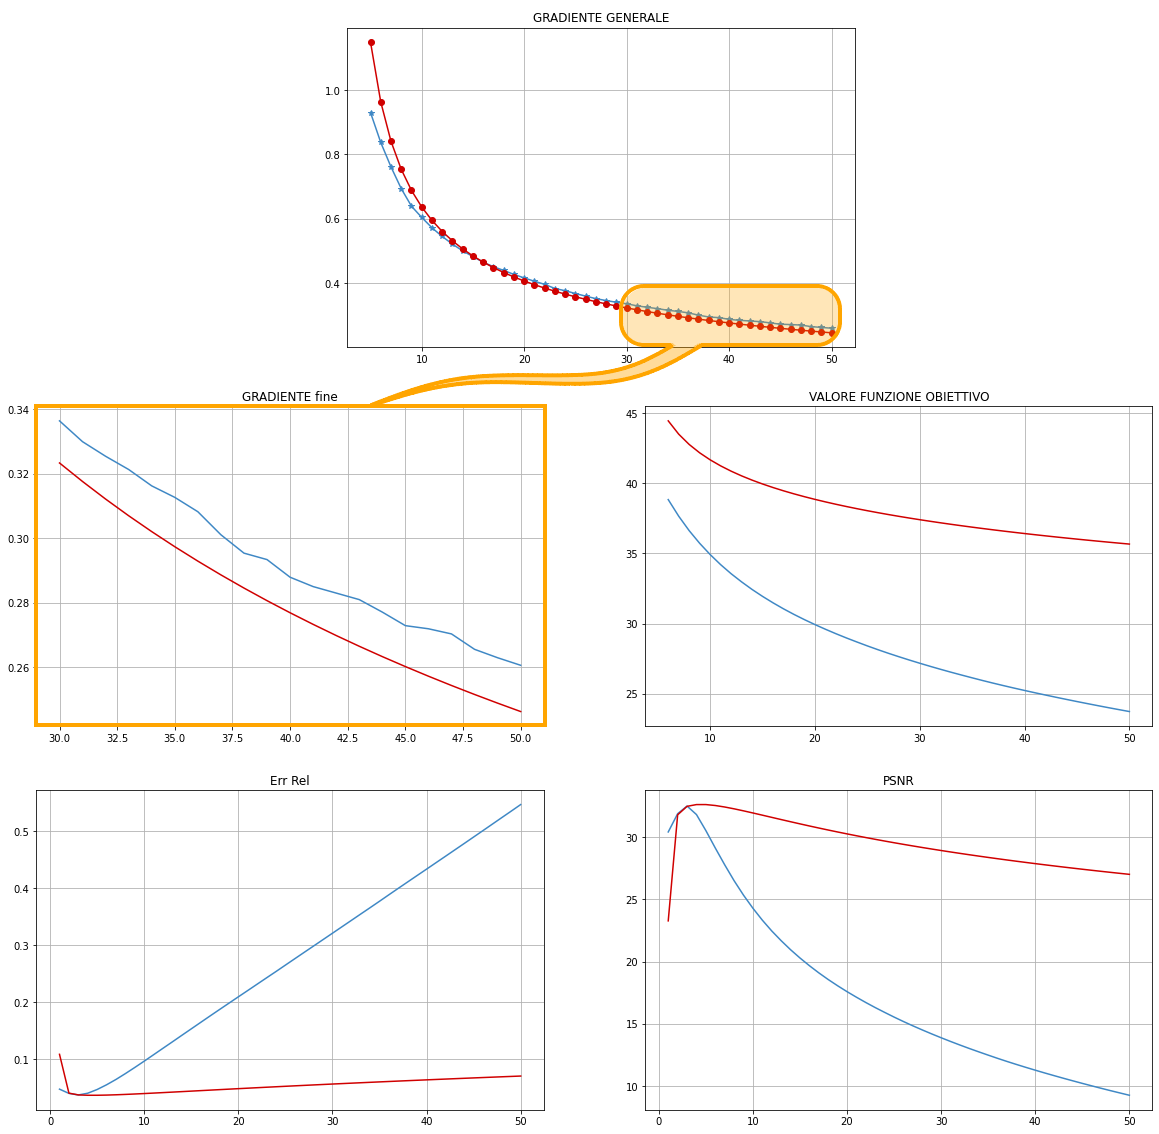
\includegraphics[width=\textwidth]{output/MGCvsMG-pugile-enph.png}
    \caption{Gradiente immagine fotografica}
    \label{fig:MGCvsMG-pugile}
\end{figure}

Prendendo "in prestito" il problema di ottimizzazione naive,
abbiamo "registrato" su due esecuzioni distinte (la prima su data.camera() 
(Figura \ref{fig:MGCvsMGdatacamera}) e la seconda su pugile 
(Figura \ref{fig:MGCvsMG-pugile}))
il comportamento dei metodi numerici utilizzati (in termini di numero di iterazioni, andamento 
dell'errore, della funzione obiettivo e della norma del gradiente), ottentendo un andamento 
generale comune ad entrambe le esecuzioni.

Abbiamo riscontrato che il metodo del gradiente con ricerca in linea inesatta è più veloce a
 raggiungere un intorno di un punto $x^{\star}$ tale che $\nabla f(x^{\star})=0$ rispetto al metodo del gradiente coniugato
 (come si può osservare nel focus delle ultime iterazioni dell'andamento della norma del gradiente).
 
Per questo motivo, considerando 
che i metodi di discesa sono definiti dall’iterazione \textbf{generale}
 \[x_{k+1} = x_k - a_k \nabla f(x_k)\]
 e si differenziano per la scelta della direzione di discesa e della lunghezza del passo $d_k$ e $a_k$, 
 le quali sono fortemente influenzate da $\nabla f(x_k)$ (\href{https://virtuale.unibo.it/mod/resource/view.php?id=750335}{slide Metodi di Discesa} pg 65/79 per metodo del gradiente coniugato)
allora avverrà che nel metodo del gradiente si presenterà prima una serie di iterati molto
 vicini l'uno dall'altro che si allontanano meno velocemente dalla vera soluzione, mantenendo quindi un PSNR
 quasi costante, poiché all'iterato successivo sommiamo una quantità molto piccola dal momento
 che viene moltiplicata per $\nabla f(x)$ la quale è molto vicino a 0. 

Dall'altra parte, l'andamento della funzione obiettivo nel metodo del gradiente coniugato è 
più ripido poiché raggiunge meno velocemente un intorno dove $\nabla f(x^{\star}) = 0$ quindi si allontana di più
 dalla vera soluzione, con ripercussioni sul PSNR ed errore relativo.